\paragraph{Tukey-Anscombe Plots (Residual Plots), Testing Whether $E(\varepsilon) = 0$}
	These plots plot the residuals versus the predicted values.
	
	\textbf{The model fits the data well} if the residuals scatter evenly around te $r=0$ line
	
	\RCode
	{
		Creating a Tukey-Anscombe Plot
	}
	{
		sections/RegressionAnalysis/ResidualAnalysis/DiagnosticsInstruments/TukeyAnscombe/Code.R
	}
	
	\begin{figure}[H]\centering
		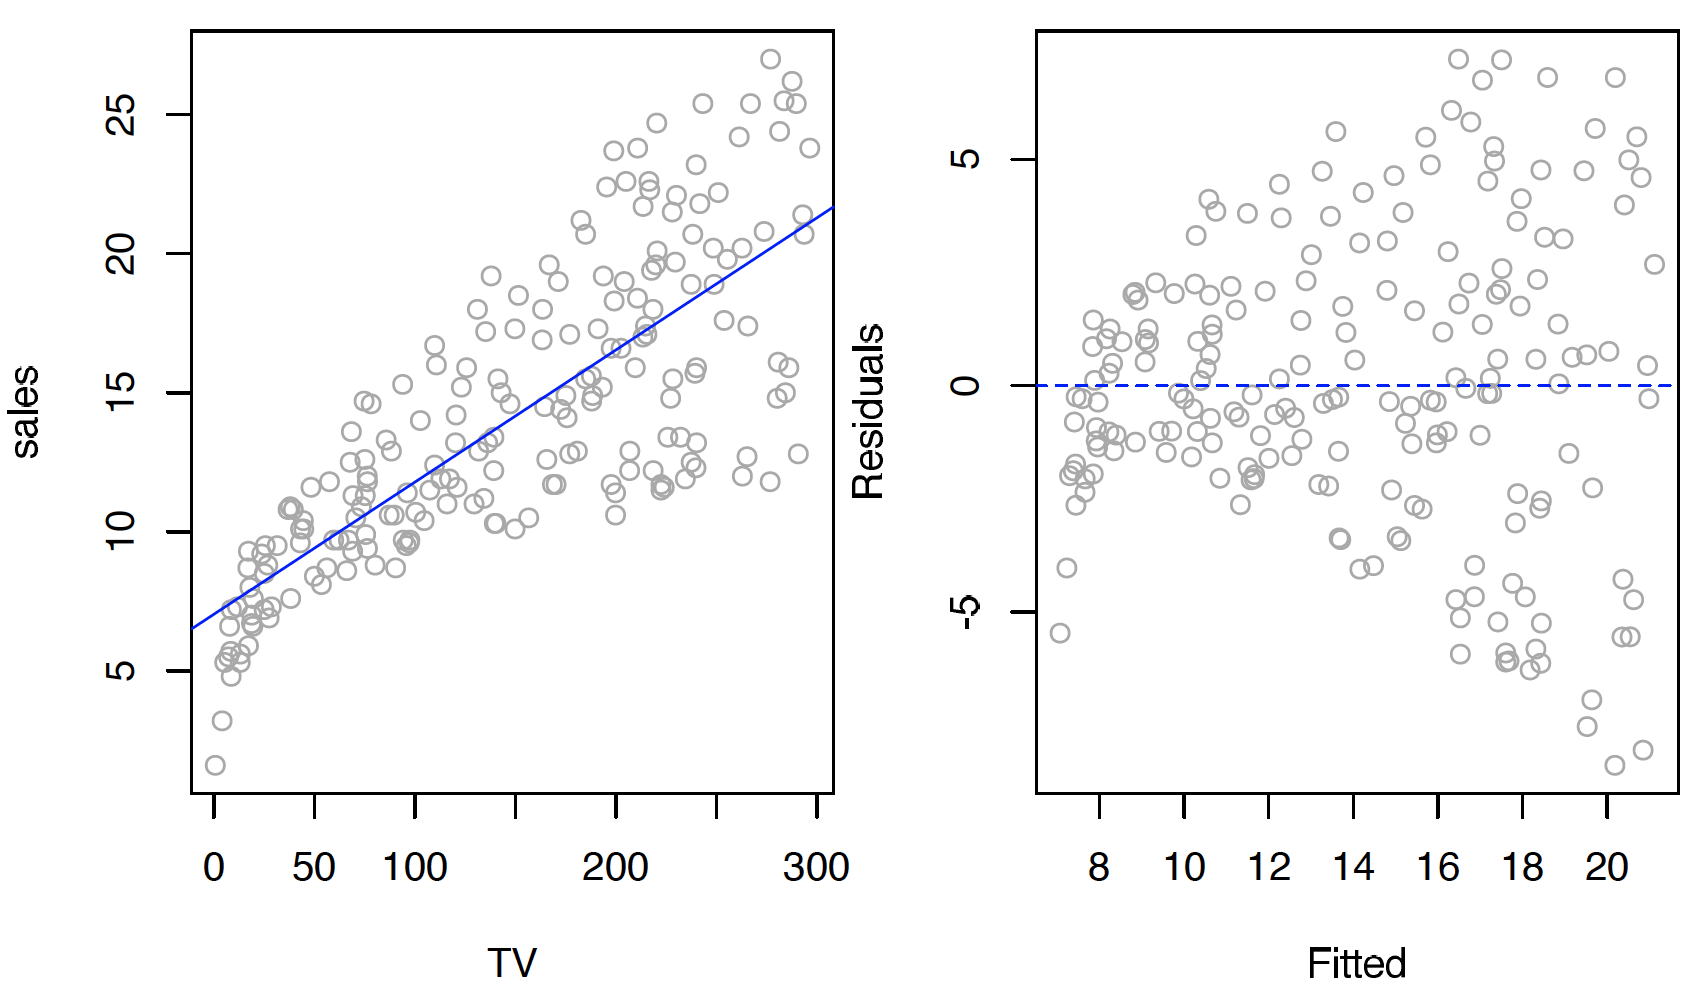
\includegraphics[width=0.8\linewidth]{images/TukeyAnscombe.png}
		\caption{Left : Scatter plot. Right: Plots of residuals versus predicted (or fitted) values (Tukey-Anscombe Plot).}
	\end{figure}